%%%%%%%%%%%%%%%%%%%%%%%%%%%%%%%%%%%%%%%%%%%%%%%%%%%%%%%%%%%%%%%%%%%%%%
% Overleaf (WriteLaTeX) Example: Molecular Chemistry Presentation
%
% Source: http://www.overleaf.com
%
% In these slides we show how Overleaf can be used with standard 
% chemistry packages to easily create professional presentations.
% 
% Feel free to distribute this example, but please keep the referral
% to overleaf.com
% 
%%%%%%%%%%%%%%%%%%%%%%%%%%%%%%%%%%%%%%%%%%%%%%%%%%%%%%%%%%%%%%%%%%%%%%
% How to use Overleaf: 
%
% You edit the source code here on the left, and the preview on the
% right shows you the result within a few seconds.
%
% Bookmark this page and share the URL with your co-authors. They can
% edit at the same time!
%
% You can upload figures, bibliographies, custom classes and
% styles using the files menu.
%
% If you're new to LaTeX, the wikibook is a great place to start:
% http://en.wikibooks.org/wiki/LaTeX
%
%%%%%%%%%%%%%%%%%%%%%%%%%%%%%%%%%%%%%%%%%%%%%%%%%%%%%%%%%%%%%%%%%%%%%%

\documentclass{beamer}

% For more themes, color themes and font themes, see:
% http://deic.uab.es/~iblanes/beamer_gallery/index_by_theme.html
%
\mode<presentation>
{
  \usetheme{Madrid}       % or try default, Darmstadt, Warsaw, ...
  \usecolortheme{default} % or try albatross, beaver, crane, ...
  \usefonttheme{serif}    % or try default, structurebold, ...
  \setbeamertemplate{navigation symbols}{}
  \setbeamertemplate{caption}[numbered]
} 

\usepackage[english]{babel}
\usepackage[utf8x]{inputenc}
\usepackage{chemfig}
\usepackage[version=3]{mhchem}

% On Overleaf, these lines give you sharper preview images.
% You might want to `comment them out before you export, though.
\usepackage{pgfpages}
\pgfpagesuselayout{resize to}[%
  physical paper width=8in, physical paper height=6in]

% Here's where the presentation starts, with the info for the title slide
\title[]{Fish recognition using deep convolutional neural network and data augmentation}
\author{Zhibin Yu}
\institute[OUC]{Ocean University of China}
\date{July 20,2017}

\begin{document}

\begin{frame}
  \titlepage
\end{frame}

% These three lines create an automatically generated table of contents.
\begin{frame}{Outline}
  \tableofcontents
\end{frame}

\section{Introduction}
\begin{frame}{Introduction}
\begin{itemize}
  \item A sub topic of computer vision and fishery industry
  \item Main difficulties
  \item You can also find more quick tips and tricks on the help pages at \url{www.overleaf.com/help}
\end{itemize}
\begin{center}\small\setatomsep{1.5em}
\schemestart
  \chemfig{*6(=-*6(-\chembelow{N}{H}-NH_2)=-=-)}
  \+
  \chemfig{(=[:-150]O)(-[:-30]R_2)-[2]-[:150]R_1}
  \arrow(.mid east--.mid west){->[\chemfig{H^+}]}
  \chemfig{*6(-=*5(-\chembelow{N}{H}-(-R_2)=(-R_1)-)-=-=)}
\schemestop
\end{center}
\end{frame}


\subsection{The importance of fish recognition}
\begin{frame}{The importance of fish recognition}

\begin{itemize}
  \item significant application of computer vision in fish survey
  \item Benefit the develop of the marine resources
  \item The needs of aquaculture and fishery
\end{itemize}

\end{frame}


\subsection{The main difficulties of fish recognition}
\begin{frame}{The main difficulties}
\begin{itemize}
  \item Various kinds of fish
  \item Complex background of images
  \item Small fish region
\end{itemize}
\begin{center}
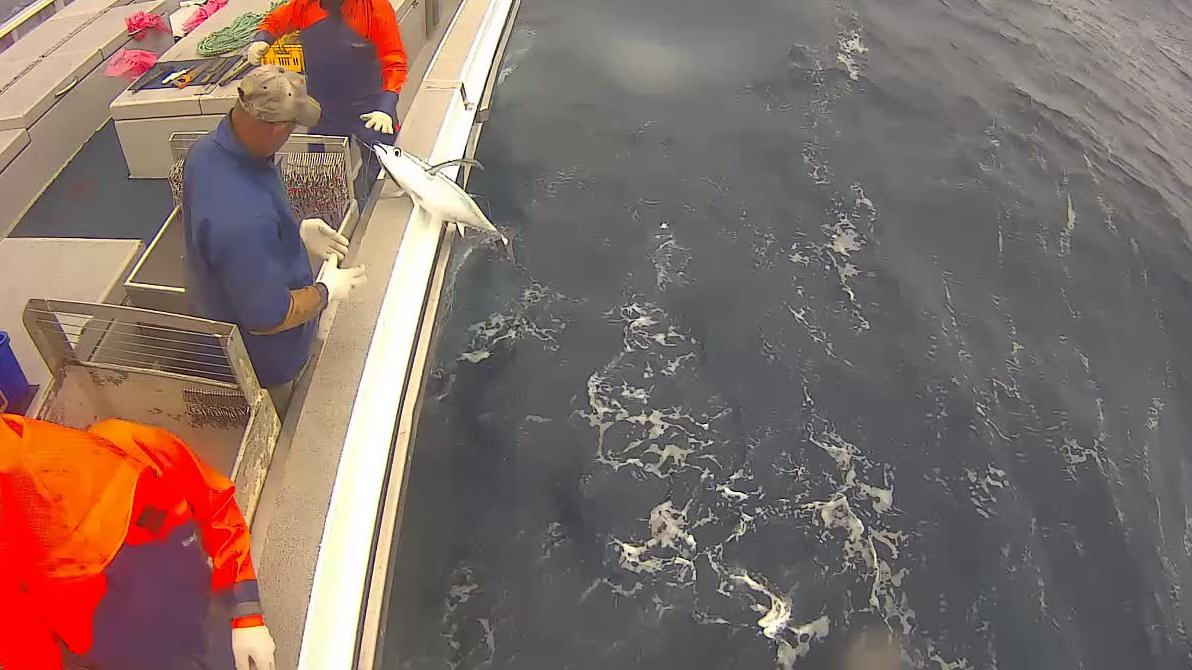
\includegraphics[width=0.8\linewidth]{1.jpg}
\end{center}
\end{frame}









\section{Using chemistry packages with \LaTeX{}}

\subsection{Chemical equations with \texttt{mhchem}}

\begin{frame}[fragile]
\frametitle{Chemical equations with \texttt{mhchem}}

\begin{itemize}
\item The \texttt{mhchem} package lets you write chemical equations in \LaTeX{} with the minimum of effort. 
\item The example below shows how the standard representation of a reaction (on the left) is created from the simple code on the right:
\end{itemize}

\begin{center}
\ce{CO2 + C -> 2CO} is created with \verb|\ce{CO2 + C -> 2CO}|
\end{center}

\begin{itemize}
\item More complicated reactions are still easy to write:
\end{itemize}

\begin{center}
\ce{SO4^2- + Ba^2+ -> BaSO4 v}\\[0.1cm]
is created with\\[0.1cm]
\verb|\ce{SO4^2- + Ba^2+ -> BaSO4 v}|
\end{center}

\end{frame}

\subsection{Getting started with some \texttt{chemfig} coffee}

\begin{frame}[fragile]
\frametitle{Getting started with some \texttt{chemfig} coffee}

It's easy to use the \texttt{chemfig} package for drawing complex molecules:

\vskip 0.5cm

\begin{center}\small\setatomsep{2.0em}
\schemestart  
\chemfig{*6((=O)-N(-CH_3)-*5(-N=-N(-CH_3)-=)--(=O)-N(-H_3C)-)}
\schemestop
\end{center}

This is the caffeine molecule, represented clearly and neatly, and built from a single line of text: \small{\verb|\chemfig{*6((=O)-N(-CH_3)-*5(-N=-N(-CH_3)-=)--(=O)-N(-H_3C)-)}|}\\[0.3cm]

If that looks quite daunting, we can learn from simpler molecules\dots{}how about a single water molecule?

\end{frame}

\subsection{Experiments with water and rings}

\begin{frame}[fragile]
\frametitle{Experiments with water and rings}

To see how the \texttt{chemfig} package creates the drawings from your code, let us look at the simple water molecule:

\vskip 0.3cm
\begin{center} 
\chemfig{H_2O} is created with \verb|\chemfig{H_2O}|
\end{center}

The simple \LaTeX{} code on the right is automatically converted into the molecular formula for water on the left. 
\vskip 0.3cm
Rings are similarly easy to code - consider the examples below:

\vskip 0.3cm

\chemfig[][scale=0.5]{A*5(-B-C-D-E-)} = \verb|\chemfig{A*5(-B-C-D-E-)}|

\vskip 0.3cm

\chemfig[][scale=0.5]{*6(=-=-=-)} = \verb|\chemfig{*6(=-=-=-)}|


\end{frame}

\section{Where to go next\dots{}}

\begin{frame}{Where to go next\dots{}}

\begin{itemize}
\item This short example was designed to introduce you to using Overleaf for scientific presentations.
\item This is made possible by the many great packages that have been developed for \LaTeX{}, including the two we focused on here (plus the \texttt{Beamer} package used for the overall presentation style). 
\item For more help on using \LaTeX{}, see the links on the Overleaf help page: \url{www.overleaf.com/help} or check out our free introductory course: \url{www.overleaf.com/blog/7}.
\end{itemize}

\begin{center}
Follow @overleaf on Twitter for all the latest news and updates.\\[0.3cm]
Happy \LaTeX ing!
\end{center}

\end{frame}

\end{document}
